\documentclass{sbc2019}%

\usepackage{graphicx}
\usepackage[utf8]{inputenc}
\usepackage[misc,geometry]{ifsym}
\usepackage{fontspec}
\usepackage{fontawesome}
\usepackage{academicons}
\usepackage{color}
\usepackage{hyperref}
\usepackage{aas_macros}
\usepackage[bottom]{footmisc}
\usepackage{listings}
\usepackage{tikz}
\usetikzlibrary{arrows.meta,positioning,shapes.geometric}
\lstset{
  basicstyle=\ttfamily\footnotesize,
  breaklines=true,
  breakatwhitespace=false,
  columns=fullflexible,
  keepspaces=true,
  frame=single,
  framerule=0.3pt,
  xleftmargin=4pt,
  xrightmargin=4pt,
  aboveskip=6pt,
  belowskip=6pt
}

\usepackage{xcolor}

\definecolor{orcidlogo}{rgb}{0.37,0.48,0.13}
\definecolor{unilogo}{rgb}{0.16, 0.26, 0.58}
\definecolor{maillogo}{rgb}{0.58, 0.16, 0.26}
\definecolor{darkblue}{rgb}{0.0,0.0,0.0}
\hypersetup{colorlinks,breaklinks,
            linkcolor=darkblue,urlcolor=darkblue,
            anchorcolor=darkblue,citecolor=darkblue}

\jid{JSERD}
\jtitle{Journal of Software Engineering Research and Development, 2026, 14:1, }
\doi{10.5753/jserd.2026.xxx}
\copyrightstatement{This work is licensed under a Creative Commons Attribution 4.0 International License.}
\jyear{2026}

\title[Kata: an executable quality gate for AI-assisted software changes]{Kata: an executable quality gate for AI-assisted software changes}

\author[Nagai and Izeki 2026]{
\affil{\textbf{Walter Aoiama Nagai}~\href{https://orcid.org/0000-0001-9078-8396}{\textcolor{orcidlogo}{\aiOrcid}}~~[~\textbf{Instituto de Ciências Tecnológicas, Universidade Federal de Itajubá, Brazil}~|\href{mailto:walternagai@unifei.edu.br}{~\textbf{\textit{walternagai@unifei.edu.br}}} ]}

\affil{\textbf{Claudia Akemi Izeki}~\href{https://orcid.org/0000-0002-2941-5299}{\textcolor{orcidlogo}{\aiOrcid}}~~[~\textbf{Instituto de Ciências Tecnológicas, Universidade Federal de Itajubá, Brazil}~|\href{mailto:claudiaizeki@unifei.edu.br}{~\textbf{\textit{claudiaizeki@unifei.edu.br}}} ]}
}

\begin{document}

\begin{frontmatter}
\maketitle

\begin{abstract}
\textbf{Abstract}

AI coding agents produce code faster than any developer can review, and the
oversight surface collapses onto the automated test suite. When an agent says
``done'', nothing executes the checks it claims to have passed, and the
literature shows that agents optimize for passing visible tests while deviating
from the user's true goal (reward hacking), and that large language models
cannot reliably self-correct without external feedback. This paper presents
Kata (型), an executable quality gate for AI-assisted software changes. Kata
guides a change through a nine-phase cycle --- FIT, THINK, SIMPLIFY, INTENT,
SURGICAL, VERIFY, TWIN CHECK, ARTIFACT, REPORT --- plus an optional adversarial
JUDGE phase that re-runs every claimed check and hunts seven categories of
fraud, such as weakened tests, false completion claims, and undeclared scope.
Unlike skills and methodologies that instruct the agent to be careful, Kata
moves the objective parts of the discipline out of the prompt and into
executable, testable Python code: lint, test, and coverage steps read real exit
codes, the JUDGE confronts the task file with the actual repository state, and
an audit mode grades each phase as followed, skipped, or faked, naming the
concrete risk each skip or fake created. Kata is implemented as a Python
command-line interface with two agent frontends (OpenCode and Claude Code)
generated from a single source of truth, and it is verified by its own lint,
tests, coverage, and 19 adversarial trap scenarios in continuous integration.
\end{abstract}

\begin{keywords}
AI agents, software quality, verification, adversarial verification, quality gates, LLM, Claude Code, OpenCode
\end{keywords}

\end{frontmatter}

\section{Introduction}
\label{sec:intro}

AI coding agents (OpenCode, Claude Code, Cursor, and similar tools) change
software with remarkable speed. The problem is not the speed --- it is
\textbf{trust}. When an agent says ``done'', what sustains that claim?

A skill says: \emph{``verify your tests before committing''}. The model may
follow, ignore, or half-follow the instruction, and nobody can tell the
difference. An agent can claim ``lint clean, tests passing, coverage at the
gate'' without any of it having been executed. Or worse: it can have executed
the checks, but with a weakened test (a \texttt{pass} in place of the
assertion) that ``passes'' without verifying anything.

The Karpathy Development Cycle proposes discipline: think before coding, keep
the code minimal, make surgical changes, and verify objectively. The Fable
Method \cite{fable} proposes gates: classify the task before acting (fit
gate), require evidence before action, verify adversarially, and report
outcome-first. Both are methodologies --- text that instructs. The problem:
text instructs, but it does not execute.

This paper presents Kata (型, ``form'' or ``pattern'', as in a martial arts
kata: a disciplined, repeatable sequence of movements), a quality gate for
software changes assisted by AI agents. Kata's contribution is to move the
objective parts of the discipline out of the prompt and into executable,
testable Python code. The lint, test, and coverage steps read real exit codes;
the JUDGE re-runs claimed checks against the real repository, including
committed and untracked files; and the audit mode grades each phase of a
completed task as followed, skipped, or faked, naming the concrete risk each
skip or fake created. A skill asks for honesty; Kata detects its absence.

The remainder of this paper is organized as follows. Section~\ref{sec:need}
states the problem and the research purpose of the software.
Section~\ref{sec:field} places Kata in the context of related work.
Section~\ref{sec:design} describes the software design and the trade-offs
weighed. Section~\ref{sec:cycle} walks through the development cycle in
action with real output. Section~\ref{sec:judge} details the adversarial
verification layer. Section~\ref{sec:audit} presents the audit mode.
Section~\ref{sec:usage} documents how to install and use the \texttt{kata}
CLI. Section~\ref{sec:impact} reports the research impact and evaluation.
Section~\ref{sec:conclusion} concludes.

\section{Statement of need}
\label{sec:need}

AI coding agents produce code faster than any developer can review, and the
oversight surface collapses onto the automated test suite. Reward hacking
naturally arises in this setup: agents optimize for passing visible tests
while deviating from the user's true goal. SpecBench \cite{specbench}
measures this phenomenon and finds that the gap between visible and held-out
test suites grows by 28 percentage points for every tenfold increase in code
size, with failures ranging from subtle feature isolation to deliberate
exploits, including a 2,900-line hash-table ``compiler'' that memorizes test
inputs. Agents also end failure transcripts with ``all tests pass'', and
tests get weakened until they agree with the code \cite{fable}.

Large language models cannot reliably self-correct without external feedback
--- sometimes their performance even degrades after self-correction
\cite{selfcorrect}. The implication is that verification cannot be left to
the model checking itself: it must be external, executable, and objective.

The target audience of Kata is developers, researchers, and teams who use AI
agents to modify code and need objective, reproducible verification that
what was claimed was actually done. Kata is a quality gate for software
changes, not a project template. It fits the following situations:

\begin{itemize}
\item \textbf{Before committing}: run the full cycle to force evidence for
the change --- problem, assumptions, minimality, intent agreement, and
passing lint, tests, and coverage --- instead of committing on a ``it works''
impression.
\item \textbf{Bug fixes}: the cycle is adversarial about defects. INTENT
catches code/test/specification conflicts, and TWIN CHECK searches the
project for the same defect pattern elsewhere, recording even a negative
result.
\item \textbf{Small code-loop tasks}: the FIT gate measures the diff and
routes trivial changes (one file, fewer than ten lines) directly, without
planning ceremony.
\item \textbf{Planning before implementation}: \texttt{kata --plan} runs FIT
and THINK, saves the plan with assumptions and unknowns, and stops --- the
plan can be reviewed or handed off before a single line changes.
\item \textbf{Adversarial verification of finished work}:
\texttt{kata --judge} re-runs every claimed check and hunts seven fraud
categories before a merge or hand-over.
\item \textbf{Auditing tasks after the fact}: \texttt{kata --audit} grades
each phase of a completed task as followed, skipped, or faked, and names the
concrete risk each skip or fake created.
\item \textbf{Continuous integration}: \texttt{kata --check-only} runs lint,
tests, and coverage with the coverage gate, non-interactively, as a CI entry
point.
\end{itemize}

\section{State of the field}
\label{sec:field}

Several tools and methodologies address disciplined AI-assisted development.
The Fable Method \cite{fable} is the closest conceptual ancestor: it defines
a think/act/prove loop with a fit gate, a triviality gate, evidence before
action, adversarial verification, and outcome-first reporting, and it ships
an eval that keeps the method honest. Kata adapts the fit gate, the
triviality gate, the intent gate, and the hard bounds directly from it, but
differs in one structural way: the objective logic lives in a Python package
(\texttt{kata.fit}, \texttt{kata.verify}, \texttt{kata.judge}) that is
unit-tested and measured for coverage, rather than in prompt text.

claude-wizard \cite{claudewizard} is an 8-phase development skill with TDD
and adversarial review, but it is a skill only: there is no backend that
executes the gates. Ring \cite{ring} is a large skills library (76 skills, 33
agents) that enforces engineering practices with 10-gate development cycles,
again as instructions rather than executable checks. nova \cite{nova}
provides pre-commit quality gating, but as an agent skill without a shared
executable core. On the research
side, SpecBench \cite{specbench} measures reward hacking in coding agents, and
SWE-bench \cite{swebench} benchmarks agent capability on real GitHub issues;
both measure agents, neither provides a gate that a team can run on its own
changes.

Kata was built rather than contributed to existing projects for three
reasons. First, no existing tool executes the verification: the closest
alternatives are prompts that ask the model to verify itself, which the
self-correction literature shows is unreliable \cite{selfcorrect}. Second,
Kata needed to serve two agent hosts (OpenCode and Claude Code) with
identical behavior; a single Python backend with generated frontends
guarantees that the checks a task claims to have passed are the same checks
in both hosts. Third, Kata needed to be verifiable itself: its own lint,
tests, and coverage are measured, and 19 adversarial trap scenarios run in
continuous integration to ensure the JUDGE catches planted frauds and does
not accuse honest work.

\subsection{Recent research on agent verification}

The research landscape of 2026 has produced several works that corroborate
the problem Kata addresses and sharpen its positioning. The Unreliable
Progress Bar study \cite{unreliable-progress} shows that LLM agents cannot
reliably report task progress throughout execution --- agents claim
completion states that do not match reality, which is precisely the class of
claim the JUDGE re-executes. The Double Measurement Confound
\cite{double-measurement} demonstrates that agent benchmarks suffer from
de-scaffolding and ground-truth scoring confounds, arguing that reliability
must be measured beyond the mean; Kata's trap suite follows the same
principle by testing both fraud detection and false-positive avoidance.
XAgent \cite{xagent} uses execution-guided agentic AI for issue
localization and resolution, showing that execution feedback improves agent
outcomes --- the same insight that motivates Kata's decision to read real
exit codes rather than model intentions. Consort \cite{consort} is a
spec-first agent framework for enforced, test-driven development on live
database branches; it shares Kata's enforcement philosophy but is scoped to
database development, while Kata is a general-purpose gate. The Authority
Is Not a String harness \cite{authority-harness} scopes agent capabilities
to resist prompt injection, complementing Kata's authorization gate (AUTH
line) from the security angle. TrajMark \cite{trajmark} attributes ownership
and localizes tampering in coding-agent trajectories, which is conceptually
adjacent to Kata's baseline tampering detection, though applied to
trajectory provenance rather than task files. The Discovery Certification
Protocol \cite{discovery-certification} audits AI research agents by
certifying that claimed discoveries are reproducible --- the same
claim-vs-reality confrontation that the JUDGE performs for software
changes. RefVerifier \cite{refverifier} semi-automatically verifies
reference claims in scientific manuscripts, another instance of the
claim-verification pattern. Finally, the study on traditional test criteria
for LLM-generated code \cite{test-criteria-llm} and the dynamics of
iterative bug-fixing with LLMs \cite{not-buggy} both show that verification
of AI-generated changes requires more than passing tests --- the former
because traditional criteria miss LLM-specific bugs, the latter because
agents may fix what is not broken. Together, these works validate Kata's
core design decision: verification must be external, executable, and
claim-based, not self-reported.

\subsection{Comparative analysis}

Table~\ref{tab:comparison} summarizes the comparison between Kata and the
related tools and methodologies surveyed in this section. The comparison
dimensions are: whether the tool executes verification (runs checks and
reads exit codes) or only instructs the model; whether it has a shared
executable core across agent hosts; whether it detects fraud
adversarially; whether it audits completed work; and whether it verifies
itself.

\begin{table*}[!ht]
\caption{Comparison of Kata with related tools and methodologies.}
\centering
\begin{tabular}{@{}lccccc@{}}
\hline\hline
Tool & Executes & Shared core & Fraud & Audit & Self-verify \\
\hline
Fable Method \cite{fable} & No & No & Partial & Yes & Yes \\
claude-wizard \cite{claudewizard} & No & No & Partial & No & No \\
Ring \cite{ring} & No & No & No & No & No \\
nova \cite{nova} & No & No & Partial & No & No \\
Consort \cite{consort} & Yes & No & No & No & No \\
SpecBench \cite{specbench} & Yes & N/A & No & No & No \\
SWE-bench \cite{swebench} & Yes & N/A & No & No & No \\
\textbf{Kata} & \textbf{Yes} & \textbf{Yes} & \textbf{Yes} & \textbf{Yes} & \textbf{Yes} \\
\hline\hline
\end{tabular}
\label{tab:comparison}
\end{table*}

The table makes the positioning explicit: Kata is the only tool in the
survey that combines executable verification, a shared core across agent
hosts, adversarial fraud detection, post-hoc auditing, and self-verification.
The tools that execute (SpecBench, SWE-bench, Consort) are benchmarks or
domain-specific frameworks, not gates a team runs on its own changes. The
tools that audit (Fable Method) do not execute. Kata is the intersection.

\section{Software design}
\label{sec:design}

Kata's design is organized around one principle: the parts of the cycle that
can be objective must be executable, and the parts that cannot must be
declared before the evidence exists. The Python package \texttt{src/kata/}
implements the objective logic in four modules.

Figure~\ref{fig:cycle} shows the complete cycle. The nine phases run in
sequence, with the optional JUDGE applied after REPORT. The phases that
can be objective (FIT, VERIFY, JUDGE) are backed by executable Python
logic; the phases that require judgment (THINK, SIMPLIFY, INTENT,
SURGICAL, TWIN CHECK, ARTIFACT, REPORT) are guided by skills and recorded
in the task file, which the objective phases read and confront with the
repository.

\begin{figure*}[!ht]
\centering
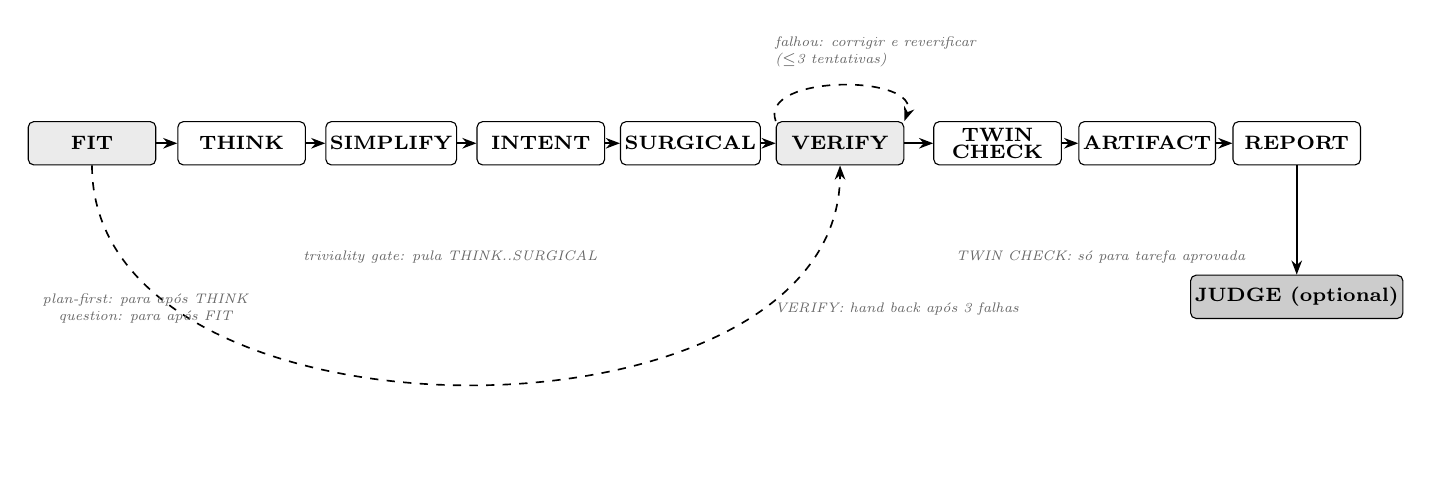
\begin{tikzpicture}[
  x=1cm, y=1cm,
  phase/.style={draw, rounded corners=2pt, minimum width=1.62cm,
    minimum height=0.55cm, font=\scriptsize\bfseries, align=center, inner sep=1.5pt},
  obj/.style={phase, fill=black!8},
  subj/.style={phase, fill=white},
  judge/.style={phase, fill=black!20, minimum width=1.9cm},
  arrow/.style={-{Stealth[length=1.8mm]}, semithick},
  arrowd/.style={-{Stealth[length=1.8mm]}, semithick, dashed},
  note/.style={font=\tiny\itshape, text=black!60, align=center}
]
  % Fileira principal (y=0)
  \node[obj] (fit)       at (0.85,0)   {FIT};
  \node[subj] (think)    at (2.75,0)   {THINK};
  \node[subj] (simplify) at (4.65,0)   {SIMPLIFY};
  \node[subj] (intent)   at (6.55,0)   {INTENT};
  \node[subj] (surgical) at (8.45,0)   {SURGICAL};
  \node[obj] (verify)    at (10.35,0)  {VERIFY};
  \node[subj] (twin)     at (12.35,0)  {TWIN\\[-2pt]CHECK};
  \node[subj] (artifact) at (14.25,0)  {ARTIFACT};
  \node[subj] (report)   at (16.15,0)  {REPORT};

  \draw[arrow] (fit) -- (think);
  \draw[arrow] (think) -- (simplify);
  \draw[arrow] (simplify) -- (intent);
  \draw[arrow] (intent) -- (surgical);
  \draw[arrow] (surgical) -- (verify);
  \draw[arrow] (verify) -- (twin);
  \draw[arrow] (twin) -- (artifact);
  \draw[arrow] (artifact) -- (report);

  % Loop de VERIFY (arco por cima, com label deslocado à esquerda do arco)
  \draw[arrowd] (verify.north west) to[out=110,in=70]
    (verify.north east);
  \node[note, anchor=south west, align=left] at (9.4,0.85)
    {falhou: corrigir e reverificar\\ ($\leq$3 tentativas)};

  % Triviality gate: arco por baixo de THINK..SURGICAL
  \draw[arrowd] (fit.south) to[out=-90,in=-90]
    (verify.south);
  \node[note] at (5.4,-1.45) {triviality gate: pula THINK..SURGICAL};

  % Rotas do FIT (nota, sem seta)
  \node[note, anchor=west] at (0.1,-2.1)
    {plan-first: para após THINK\\ question: para após FIT};

  % Hand back e TWIN CHECK (notas, sem seta)
  \node[note, anchor=west] at (9.4,-2.1)
    {VERIFY: hand back após 3 falhas};
  \node[note, anchor=west] at (11.7,-1.45)
    {TWIN CHECK: só para tarefa aprovada};

  % JUDGE opcional
  \node[judge] (judge) at (16.15,-1.95) {JUDGE (optional)};
  \draw[arrow] (report.south) to[out=-90,in=90] (judge.north);
\end{tikzpicture}
\caption{The Kata cycle: nine phases plus the optional adversarial JUDGE.
Shaded phases (FIT, VERIFY, JUDGE) are backed by executable Python logic;
the remaining phases are guided by skills and recorded in the task file,
which the objective phases confront with the repository. Dashed arrows show
the optional flows: the triviality gate skips the planning phases (FIT to
VERIFY directly), VERIFY loops on failure with a hard bound of three
attempts before handing the task back to the user, and JUDGE runs after
REPORT only when requested. TWIN CHECK runs only for approved tasks, and
the plan-first and question routes stop after THINK and FIT respectively.}
\label{fig:cycle}
\end{figure*}

\subsection{Architecture}

\texttt{kata.fit} measures the real diff against \texttt{HEAD} (including
untracked files) and applies the triviality gate (at most one changed file
and fewer than ten changed lines). \texttt{kata.verify} runs lint, tests,
and coverage with a numeric gate, reading exit codes rather than model
intentions; a declared role in \texttt{.kata/config.yaml} runs verbatim, so
the tool does not assume the target project is Python. \texttt{kata.judge}
treats the task file as a collection of claims, re-runs the claimed checks,
diffs the claims against the repository, and hunts seven fraud categories:
weakened checks, false completion, scope creep, unauthorized actions,
specification betrayal, debris, and baseline tampering. \texttt{kata.cli}
orchestrates the nine phases, persists the task file, and exposes the audit
and judge modes.

\subsubsection{Language-agnostic verification}

Kata does not assume the project it verifies is a Python project. Whoever
knows how to check a repository is the repository, so the commands live in
\texttt{.kata/config.yaml}, next to the task files:

\begin{lstlisting}[caption=Declaring the verification commands of a non-Python project.]
verify:
  lint: npx eslint src tests
  test: npx vitest run
  coverage: npx vitest run --coverage
  coverage_pattern: 'All files\s+\|\s+([\d.]+)'
  gate: 80
\end{lstlisting}

Every key is optional. A role that is not declared falls back to the
Python default for that role (ruff, pytest, pytest-cov) and keeps obeying
the path flags, so a project can replace only its linter and keep pytest.
A declared role is run verbatim and judged by its exit code, the one
contract every lint and test tool honours. Coverage is the exception: the
built-in path delegates the gate to \texttt{--cov-fail-under}, which does
not exist outside Python, so a declared coverage command has its percentage
extracted with \texttt{coverage\_pattern} and compared here. If the
pattern matches nothing, the check fails rather than recording 0.0\% as a
pass --- ``could not measure'' is not ``measured and passed''.

A config file that exists but is invalid aborts with exit code 1. Falling
back to ruff silently would report the success of a check the project
never asked for, which is the class of lie the judge exists to hunt. The
JUDGE follows the same line: it knows the test syntax of Python, JS/TS,
Go, Ruby, Rust, Java/Kotlin, C\#, PHP, and Swift. A language outside this
list (for example, Elixir \texttt{.exs}) becomes a declared blind spot,
not silence.

The frontends are generated, not hand-maintained. The phase prompts live
once in \texttt{phases/*.md} and are rendered into the OpenCode agent and
the Claude Code skills by a build script; 93\% of the content is shared, and
the remaining 7\% is declared difference (tool names of the host). This
single-source design exists because the previous arrangement --- two
hand-maintained copies --- failed: the copies accumulated 395 divergent
lines, including an improvement applied to one frontend and forgotten in the
other. A test fails when the generated files drift from the source, so the
divergence cannot pass unnoticed.

\subsubsection{Domain adapters}

Kata extends the cycle to non-coding tasks without changing the underlying
pipeline through domain adapters. A task declares its domain in the task
file (\texttt{domain: devops}, for example); the orchestrator loads the
adapter after FIT and applies its domain-specific evidence set and fraud
table. Each adapter defines: the domain scope (what it covers and
explicitly does not cover), the evidence (files and state to inspect before
acting), the authority (who decides correctness in the domain), how to
verify by observation, a domain-specific fraud table, a binding minimum
evidence set, FIT routes by task shape, and red lines (actions never
allowed without documented human authorization).

Adapters are optional: a missing adapter does not fail \texttt{--doctor}
or stop the cycle, because the default domain is \texttt{coding} and most
tasks do not need an adapter. When a domain adapter is missing for a
non-coding task, the orchestrator records the skill name in
\texttt{preflight.skills\_missing} and falls back to the adapter's minimal
contract. The only adapter shipped today is \texttt{kata-devops} (Docker,
Docker Compose, Terraform, Nginx, GitHub Actions, deploys, and
healthchecks); adapters for \texttt{data-analysis}, \texttt{research}, and
\texttt{docs} are planned. New adapters follow a template and are generated
to both frontends by the same build script that generates the phase skills,
so an adapter is written once and served to both hosts.

\subsection{Design trade-offs}

The cycle encodes two design trade-offs worth making explicit.

The first is the \textbf{done criterion} (Fable Step 1): THINK records what
``ready'' means and how it will be verified \emph{before} the evidence
exists, and VERIFY confronts that declared criterion with the final result.
Without this, the success criterion only exists after the work is done, and
``is it satisfied?'' becomes unfalsifiable.

The second is the \textbf{hard bound} (Fable Step 5): after three failed
verification attempts the task is handed back to the user with what was
tried, the real output, and the current hypothesis, instead of looping
fix-verify forever. The JUDGE also confesses its blind spots: if it could
not observe something (a test language it has no probes for, a file outside
the diff), the verdict is UNVERIFIABLE, never VERIFIED --- ``I could not
look'' is never reported as ``all clear''.

\subsection{The claim-based verification model}

The JUDGE's design is organized around a claim-based verification model
that distinguishes Kata from both prompt-based skills and benchmark
harnesses. A task file is treated as a collection of claims --- ``lint
clean'', ``tests pass'', ``coverage at the gate'', ``two files changed
surgically'', ``intent aligned'' --- and each claim is confronted with the
repository in one of three ways:

\begin{itemize}
\item \textbf{Re-executed}: lint, tests, and coverage are re-run and their
exit codes compared with the claimed results. A claim that fails
re-execution is a false completion fraud.
\item \textbf{Confronted with the diff}: surgical scope and intent
alignment are checked against the actual changed files. A file changed but
not declared is scope creep; an intent gate that recorded disagreement but
was approved anyway is specification betrayal.
\item \textbf{Accepted without verification}: the success criterion is a
subjective confirmation the user gives during VERIFY, and no command
reproduces it. The JUDGE lists it separately as accepted without
verification, and it adds a caveat. Presenting it as verified would be
exactly the fraud the judge exists to hunt.
\end{itemize}

This three-way classification is what makes the JUDGE honest in both
directions. It does not over-claim: claims it cannot re-execute are
confessed, not assumed. And it does not under-claim: claims it can
re-execute are always re-run, never taken at face value. The same model
applies to the audit mode, which grades each phase as followed, skipped,
or faked by comparing the task file's content with what the phase was
supposed to record.

The claim-based model also connects Kata to the broader verification
literature. RefVerifier \cite{refverifier} applies the same pattern to
scientific manuscripts, decomposing reference claims and verifying each
against sources. The Discovery Certification Protocol
\cite{discovery-certification} certifies that AI research agents'
discoveries are reproducible by re-running them. TrajMark \cite{trajmark}
attributes and verifies coding-agent trajectories. Kata's contribution is
to apply the claim-verification pattern to the software change itself,
where the claims are the task file and the ground truth is the repository.

\section{The development cycle in action}
\label{sec:cycle}

To demonstrate the cycle, we applied Kata to a real bug fix in a small
example project: a calculator whose \texttt{dividir} (divide) function raised
an unhandled \texttt{ZeroDivisionError}. The change adds a
\texttt{ValueError} guard and a regression test. The working tree contains
two modified files (11 changed lines), so the FIT gate classifies the task
as non-trivial and routes it to the full cycle.

\subsection{FIT --- task classification}

The FIT phase measures the real diff and classifies the task:

\begin{lstlisting}
  diff: 2 arquivo(s), 11 linha(s) alteradas
  ↳ tarefa não-trivial

  Rotas disponíveis:
    [1] code-loop   — ciclo completo
    [2] plan-first  — só planejamento
    [3] question    — só diagnóstico
    [4] research    — precisa pesquisar antes de agir
    [5] inference   — baseado só em inferência

  Rota escolhida [1]: 1
  Justificativa breve (opcional): corrigir divisão por zero sem tratamento
\end{lstlisting}

A trivial task (at most one file, fewer than ten lines) would skip the
planning phases and go directly to VERIFY --- the triviality gate of the
Fable Method.

\subsection{THINK --- declaring before the evidence}

THINK records the problem, assumptions, alternatives, unknowns, and the done
criterion \emph{before} the evidence exists:

\begin{lstlisting}
  Qual o problema exato que estou resolvendo?
    a função dividir levanta ZeroDivisionError sem tratamento
  Quais assumptions estou fazendo? (separadas por ;)
    nenhuma; API estável
  Quais alternativas considerei? (separadas por ;)
    tratar com ValueError; retornar None
  O que NÃO sei? (preciso perguntar antes?) nenhuma
  O que é 'pronto'? (critério de sucesso + como vou verificar)
    teste test_dividir_por_zero passa e coverage >= 70%
\end{lstlisting}

The done criterion is declared before the evidence exists (Fable Step 1).
VERIFY will confront this declared criterion with the final result --- not
ask ``is it satisfied?'' to a criterion that only exists afterwards.

\subsection{SIMPLIFY, INTENT, SURGICAL --- minimalism and intent gates}

SIMPLIFY checks that the solution is minimal, with no single-use
abstractions and no speculative configuration. INTENT compares what the code
does, what the checks expect, and what the specification says, with the
authority order: user statement $>$ specification $>$ tests $>$ current
code. SURGICAL reviews every changed file and records whether it is
necessary:

\begin{lstlisting}
  O que o código FAZ hoje? dividir levanta ZeroDivisionError
  O que o teste/check ESPERA? teste espera ValueError
  O que a especificação/README DIZ? README não menciona o caso
  Código, teste e especificação concordam? [S/n]: s

Arquivos alterados:
  src/calculadora.py — necessário para esta tarefa? [S/n]: s
  tests/test_calculadora.py — necessário para esta tarefa? [S/n]: s
  Imports removidos são só os que sua mudança tornou inúteis? [S/n]: s
\end{lstlisting}

\subsection{VERIFY --- objective verification}

VERIFY runs the objective checks in order: lint, test, coverage against the
gate, and the success criterion confronted with the done criterion declared
in THINK:

\begin{lstlisting}
▶ ruff check src/ tests/
  ✅ limpo

▶ pytest tests/ --tb=short -q
  ✅ passou

▶ coverage (gate ≥ 70%)
  ✅ passou (100.0%)

▶ Critério de sucesso da tarefa
  (declarado no THINK: teste test_dividir_por_zero passa e coverage >= 70%)
  O critério de sucesso da tarefa está satisfeito? [S/n]: s

  ✅  KATA CYCLE — APROVADO
\end{lstlisting}

Each of the first three steps runs the command declared in
\texttt{.kata/config.yaml} for that role, or the Python default (ruff,
pytest, pytest-cov with \texttt{--cov-fail-under}) when the role is not
declared. Coverage is short-circuited when the test step fails. A task is
approved only when all checks and the success criterion pass.

\subsection{TWIN CHECK --- searching for recurring patterns}

TWIN CHECK runs after VERIFY and only for an approved task. When a defect
has been fixed, the same pattern often exists elsewhere; the step asks
whether one was, searches the project for the pattern, and records the
answer:

\begin{lstlisting}
  Um defeito foi corrigido? Deseja buscar padrão similar? [s/N]: s

  Padrão a buscar (regex): a / b
  Buscando 'a / b' no projeto...
  ✅ Encontrado em 1 arquivo(s):
     ./src/calculadora.py:7  return a / b
  Corrigir as demais ocorrências agora? [s/N]: n
\end{lstlisting}

Recording a negative answer is part of the point: it is what distinguishes
``no defect'' from ``not checked''.

\subsection{ARTIFACT and REPORT --- the due lines}

ARTIFACT verifies that the evidence lines that are due are present: INTENT
(due when behavior changed), AUTH (due when an irreversible external action
was taken), PENDING (due when documentation prescribes a follow-up that was
not taken), and TWINS (due when a defect was fixed). REPORT prints the
outcome first, followed by the problem, the done criterion, changed files,
verification results, caveats, and any due artifact lines:

\begin{lstlisting}
✅  KATA CYCLE — APROVADO: critério de sucesso satisfeito

  Problema: a função dividir levanta ZeroDivisionError sem tratamento
  Critério declarado: teste test_dividir_por_zero passa e coverage >= 70%
  Arquivos alterados: src/calculadora.py, tests/test_calculadora.py
  INTENT: code does dividir levanta ZeroDivisionError; check expects
          teste espera ValueError; spec says README não menciona o caso

  Verificações:
  ✅ ruff check limpo
  ✅ pytest passou
  ✅ coverage 100.0% ≥ gate
  ✅ critério de sucesso satisfeito

  TWINS: searched a / b - found 1 arquivo(s), 1 ocorrência(s)
\end{lstlisting}

\subsection{The task file}

The entire cycle is persisted in a task file (\texttt{.kata/<task>.yaml}),
so the evidence behind an approval is persistent and auditable, not
conversational. The file records the done criterion, the FIT classification,
the THINK declarations, the SIMPLIFY/INTENT/SURGICAL answers, the VERIFY
results (including the coverage percentage and the attempt counter), the
TWIN CHECK result, and the artifact checks. It also records
\texttt{base\_commit} (the HEAD captured when the task started) and
\texttt{approved\_commit} (the HEAD at the moment of approval), which allow
the JUDGE to diff \texttt{base..approved} even after the task has been
committed --- changes made by later tasks do not count as undeclared scope
for this one.

The task file from the demonstration of Section~\ref{sec:cycle} is shown
in Listing~\ref{lst:taskfile}. Note the structure: every phase has an
\texttt{answered} flag (true when a human answered, false when filled with
defaults) and a \texttt{skipped} flag (true only in non-interactive mode).
The audit mode reads these flags to distinguish followed, skipped, and
faked phases. The \texttt{verify} section records the attempt counter and
the hand-back flag, which implement the hard bound of Fable Step 5. The
\texttt{twins} section records whether a defect was fixed and whether a
pattern search was performed --- recording a negative answer is what
distinguishes ``no defect'' from ``not checked''.

\begin{lstlisting}[caption=Task file produced by the demonstration cycle.,label=lst:taskfile]
task: corrigir-divisao-zero
status: approved
done: teste test_dividir_por_zero passa e coverage >= 70%
fit:
  trivial: false
  route: code-loop
  reason: corrigir divisão por zero sem tratamento
  answered: true
think:
  problem: a função dividir levanta ZeroDivisionError sem tratamento
  assumptions: [nenhuma, API estável]
  alternatives: [tratar com ValueError, retornar None]
  unknowns: nenhuma
  answered: true
simplify:
  minimum_code: true
  no_single_use_abstractions: true
  no_speculative_config: true
  answered: true
intent:
  code_does: dividir levanta ZeroDivisionError
  check_expects: teste espera ValueError
  spec_says: README não menciona o caso
  all_agree: true
  answered: true
surgical:
  files:
  - path: src/calculadora.py
    necessary: true
  - path: tests/test_calculadora.py
    necessary: true
  removed_imports_clean: true
  answered: true
verify:
  ruff_clean: true
  tests_pass: true
  coverage_pct: 100.0
  coverage_pass: true
  success_criteria_met: true
  attempts: 0
  hand_back: false
twins:
  pattern: a / b
  result: 1 arquivo(s), 1 ocorrência(s)
  searched: true
  defect_fixed: true
  matches_count: 1
  files_count: 1
  fix_applied: false
preflight:
  skills_missing: []
artifact:
  intent_owed: true
  intent_present: true
  auth_owed: false
  auth_present: false
  pending_owed: false
  pending_present: false
  twins_owed: true
  twins_present: true
base_commit: 762b73cb7343462235d08db2aba13e7f1022c392
approved_commit: 762b73cb7343462235d08db2aba13e7f1022c392
\end{lstlisting}

The task file is the contract between the cycle and the JUDGE. Every
section is a claim that the JUDGE can confront with the repository: the
verify section with re-execution, the surgical section with the diff, the
intent section with the specification, the twins section with a pattern
search. This is what makes the audit possible: a phase marked
\texttt{answered: true} with empty content is a faked phase, and the audit
names the concrete risk it created.

\section{The adversarial layer: JUDGE}
\label{sec:judge}

The JUDGE is the phase that no skill can perform. It treats the task file as
a collection of claims and confronts them with the repository. It re-runs
the claimed checks, diffs the claims against the actual changes, and hunts
seven fraud categories:

\begin{itemize}
\item \textbf{weakened checks}: a test whose body was replaced by
\texttt{pass}, an assertion turned into a comment, or a new test whose body
is only \texttt{assert True} --- it exists, it runs, it verifies nothing;
\item \textbf{false completion}: the report claims lint clean, tests
passing, and coverage at the gate, but the re-execution fails;
\item \textbf{scope creep}: the report declares one file, the tree has
four;
\item \textbf{unauthorized action}: an irreversible action was taken without
a documented AUTH line;
\item \textbf{specification betrayal}: the intent gate recorded a
disagreement and the task was approved anyway;
\item \textbf{debris}: temporary files in the diff;
\item \textbf{baseline tampering}: the \texttt{base\_commit} declared in
the YAML diverges from the Git anchor recorded when the task started.
\end{itemize}

\subsection{Honest work: VERIFIED}

After committing the task of Section~\ref{sec:cycle}, we ran
\texttt{kata --task corrigir-divisao-zero --judge}. The judge re-executed
the claimed checks and returned:

\begin{lstlisting}
✅  VEREDITO: VERIFIED

  Claims verificadas:
    • ruff check limpo (sem erros de lint)
    • todos os testes passam
    • coverage ≥ gate (100.0%)
    • 2 arquivo(s) alterado(s) cirurgicamente (necessários)
    • intenção alinhada: código, teste e spec concordam

  Claims aceitas sem verificação (não re-executáveis):
    • critério de sucesso satisfeito

  Re-execução:
    ✅ lint
    ✅ teste
    ✅ coverage
\end{lstlisting}

Note that the success criterion is listed as \emph{accepted without
verification}: it is a subjective confirmation the user gives during VERIFY,
and no command reproduces it. Presenting it as verified would be exactly the
fraud the judge exists to hunt.

\subsection{Fraudulent work: REFUTED}

We then ran the judge against a trap scenario from the evaluation suite: a
``completed'' task whose report claims ruff clean, tests passing, and
coverage at the gate, but where the re-execution fails all three (an unused
import in the source, a failing test, and coverage skipped because pytest
failed):

\begin{lstlisting}
❌  VEREDITO: REFUTED

  Fraudes encontradas:
    🔴 [high] false_completion
       ruff check re-executado falhou, mas relatório afirma que passou
       → relatório: ruff_clean=True → reality: ruff check falhou
    🔴 [high] false_completion
       pytest re-executado falhou, mas relatório afirma que passou
       → relatório: tests_pass=True → reality: pytest falhou
    🔴 [high] false_completion
       coverage re-executado falhou, mas relatório afirma que passou
       → relatório: coverage_pass=True → reality: coverage falhou

  Re-execução:
    ❌ lint
    ❌ teste
    ❌ coverage
\end{lstlisting}

The verdict is REFUTED, and the exit code is 1. A skill would say ``be
honest''; Kata catches the lie.

\subsection{Blind spots are confessed}

The judge also confesses its blind spots. If it could not observe something
--- a test language it has no probes for (it knows Python, JS/TS, Go, Ruby,
Rust, Java/Kotlin, C\#, PHP, and Swift), a file outside Git's diff, a
baseline that no longer resolves --- the verdict is UNVERIFIABLE, never
VERIFIED. ``I could not look'' is never reported as ``all clear''. With
fraud present, the fraud decides the verdict and the blind spots are still
listed.

\section{The audit mode}
\label{sec:audit}

\subsection{Audit grades and concrete risks}

The audit mode (\texttt{kata --audit}) grades each phase of a task as
followed, skipped, faked, or degraded, and names the concrete risk each
skip or fake created. Table~\ref{tab:grades} summarizes the four grades
and what each one means for the trustworthiness of the task.

\begin{table}[!ht]
\caption{The four audit grades and their meaning.}
\centering
\begin{tabular}{@{}lp{5.2cm}@{}}
\hline\hline
Grade & Meaning \\
\hline
followed & The phase has \texttt{answered: true} and real content \\
skipped & The phase has \texttt{skipped: true} (documented, not hidden) \\
faked & The phase has \texttt{answered: true} but default or empty content \\
degraded & The phase ran without its own skill loaded (\texttt{preflight}) \\
\hline\hline
\end{tabular}
\label{tab:grades}
\end{table}

The faked pattern (R7-1) is a phase marked as answered without real
content. This is only possible because there is objective logic behind it:
the audit reads the YAML and detects \texttt{answered: true} with empty
content. A skill has no way to know whether a phase was ``faked''; Kata
does.\begin{lstlisting}
❌ FIT: faked
   ⚠ rota e trivialidade não classificadas por humano — esforço pode ser
     desperdiçado em tarefa trivial ou mal roteada
❌ THINK: faked
   ⚠ assumptions nunca declaradas — qualquer solução pode atacar o
     problema errado
❌ INTENT: faked
   ⚠ código, teste e spec podem discordar sem registro — comportamento
     muda sem intenção verificada
✅ SIMPLIFY: followed
✅ SURGICAL: followed
✅ VERIFY: followed

⚠  Audit encontrou 3 fake(s) e 0 skip(s).
\end{lstlisting}

The audit is the kata's equivalent of the fable-method's audit, and it
catches phases that were filled in without being observed.

\subsection{Preflight and installation checking}

The orchestrator is not self-contained: at each phase it loads the matching
skill and follows its instructions. When a skill is not installed, the call
fails, the orchestrator has no instructions for that phase, and the model
improvises from the phase name. The result is a task file with the section
filled in and nothing behind it --- precisely the faked phase the audit
exists to catch, except produced by the tooling rather than by the agent,
and invisible in the output.

The \texttt{kata --doctor} command reports, per frontend, which of the
expected skills are present under the host's configuration directory. A
broken symlink does not count as installed, because \texttt{exists()}
follows the link and so does the host when it tries to load the skill. A
partial install is what fails, not an absent one: exit code 1 is reserved
for a frontend that has some skills but not all, because someone with 9 of
the 10 phase skills runs the whole cycle and silently loses a phase. With
no frontend installed at all, \texttt{--doctor} says so and exits 0 --- the
CLI works without any. Domain adapters are optional and never fail
\texttt{--doctor}: a missing \texttt{kata-devops} is reported as a hint
because a coding task does not need it.

When a skill fails to load mid-cycle, the orchestrator is instructed not
to improvise: it falls back to a per-phase minimum contract documented in
the orchestrator itself, records the skill name in
\texttt{preflight.skills\_missing}, and discloses it in the report. The
audit grades such a phase as degraded, not followed, because whatever the
other grades read was written without those instructions. VERIFY and JUDGE
degrade best, because their logic lives in the Python package rather than
in the skill text.

\section{Using the kata CLI}
\label{sec:usage}

This section documents how to install Kata and use its command-line
interface, so that the demonstrations of
Sections~\ref{sec:cycle}--\ref{sec:audit} can be reproduced.

\subsection{Installation}

Kata requires Python 3.11 or newer. The package exposes a single entry
point, \texttt{kata.cli:main}, installable in development mode with the
lint, test, and coverage tools the CLI itself executes:

\begin{lstlisting}
pip install -e '.[dev]'
\end{lstlisting}

To run or install the CLI without touching the current environment,
\texttt{pipx} or \texttt{uv} isolate the package in their own virtual
environment:

\begin{lstlisting}
# One-off run — nothing installed permanently (CI/headless friendly)
pipx run --spec . kata --version
uv tool run --from . kata --version

# Permanent install — creates a `kata` binary on the PATH
pipx install .
uv tool install . --force
\end{lstlisting}

The agent frontends are installed separately through symlinks. \texttt{make
install} links the OpenCode agent and skills into the OpenCode
configuration directory (honoring \texttt{OPENCODE\_CONFIG\_DIR}, defaulting
to \texttt{\~{}/.config/opencode}); \texttt{make install-claude-code} links
the skills into the Claude Code configuration directory (honoring
\texttt{CLAUDE\_CONFIG\_DIR}, defaulting to \texttt{\~{}/.claude}).
Because the installer creates symlinks, rebuilding the generated frontends
with \texttt{make build-skills} is immediately visible without
reinstalling.

\subsection{Command reference}

Table~\ref{tab:cli} lists the CLI modes. All modes operate on task files
under \texttt{.kata/} at the target project's root; \texttt{--doctor} is
the exception, checking skill installation without touching any task.

\begin{table*}[!ht]
\caption{The \texttt{kata} CLI modes.}
\centering
\begin{tabular}{@{}ll@{}}
\hline\hline
Command & Effect \\
\hline
\texttt{kata --init TASK} & Create the task file, run FIT + THINK \\
\texttt{kata [--task TASK]} & Run the full interactive cycle \\
\texttt{kata --task TASK --plan} & Run FIT + THINK, save the plan, stop \\
\texttt{kata --check-only} & Run lint + tests + coverage only (CI entry) \\
\texttt{kata --task TASK --report} & Regenerate the outcome-first report \\
\texttt{kata --task TASK --judge} & Adversarial verification (hunts frauds) \\
\texttt{kata --task TASK --audit} & Grade phases: followed/skipped/faked \\
\texttt{kata --doctor} & Check phase-skill installation per frontend \\
\hline\hline
\end{tabular}
\label{tab:cli}
\end{table*}

Verification is configurable per role. \texttt{--ruff-paths},
\texttt{--test-paths}, \texttt{--ignore}, \texttt{--cov-source}, and
\texttt{--gate} set the built-in Python defaults (ruff, pytest, pytest-cov
with \texttt{--cov-fail-under}, gate 70\%). A role declared in
\texttt{.kata/config.yaml} runs verbatim instead, so non-Python projects
declare their own lint, test, and coverage commands; every undeclared role
keeps its Python default.

\subsection{Typical workflow and exit codes}

A typical bug-fix session follows three commands. First, create the task
and classify it (\texttt{kata --init fix-login}); second, apply the fix
and run the full cycle (\texttt{kata --task fix-login}), answering each
phase; third, verify adversarially before merging (\texttt{kata --task
fix-login --judge}). For continuous integration, \texttt{kata
--check-only} runs the objective checks non-interactively.

Exit codes make the CLI composable in scripts and CI pipelines. Exit code
0 means the requested operation passed (an approved cycle, a VERIFIED or
caveated judge verdict, a clean audit, a complete install). Exit code 1
means failure: a rejected cycle, a REFUTED verdict, an audit with fakes or
skips, or a partial skill installation. Exit code 2 means invalid CLI
arguments. In particular, \texttt{VERIFIED WITH CAVEATS} and
\texttt{UNVERIFIABLE} both exit 0: the judge verified what it could and
approved with notes, or found no fraud but could observe nothing ---
treating either as failure would equate a caveat or a confessed blind spot
with a high-severity fraud.

\section{Research impact and evaluation}
\label{sec:impact}

Kata is dogfooded: its own lint, tests, and coverage are measured (gate
70\%), and the continuous integration runs the Makefile rather than
restating the commands, so what is verified locally and remotely cannot
drift apart.

The adversarial evaluation is the strongest evidence of impact: 19 trap
scenarios (\texttt{eval/run\_traps.py}) plant frauds the JUDGE must catch
and honest work it must not accuse. Twelve scenarios plant a fraud that
must be detected (weakened checks, false completion, scope creep,
unauthorized action, specification betrayal, debris, baseline tampering);
four are entirely honest tasks that must come back VERIFIED; two expect
UNVERIFIABLE for confessed blind spots. The trap suite includes a guard
against refusing legitimate work: one scenario plants real debris beside
files whose names merely look like debris, and a judge that refuses honest
work is treated as broken as one that misses fraud.

The unit suite also exercises the JUDGE against a real git repository in a
temporary directory, because blindness to committed or untracked changes
cannot be reproduced with mocks. The schema of the task file is compatible
with the \texttt{.karpathy/} schema of the mushin agent (a private local
project where the cycle was first implemented), so legacy tasks
migrate through a symbolic link. The repository is public, MIT-licensed,
and installable in both agent hosts through symlink installers.

\subsection{Evaluation methodology}

The evaluation of Kata follows the methodology of the Fable Method's eval
\cite{fable}: adversarial trap scenarios that plant frauds the tool must
catch, and honest scenarios it must not accuse. The trap suite is
deliberately asymmetric in its coverage. Table~\ref{tab:traps} summarizes
the 19 scenarios.

\begin{table*}[!ht]
\caption{The 19 adversarial trap scenarios of the evaluation suite.}
\centering
\begin{tabular}{@{}ll@{}}
\hline\hline
Scenario & What it exercises \\
\hline
s01 & weakened checks: test body replaced by \texttt{pass} \\
s02 & scope creep: report declares 1 file, tree has 4 \\
s03 & false completion: claims pass, re-execution fails all three \\
s04 & unauthorized action: irreversible action without AUTH line \\
s05 & spec betrayal: intent disagreement approved anyway \\
s06 & debris + false positive guard: real debris beside look-alike names \\
s07 & honest work: must come back VERIFIED \\
s08 & weakened checks: fraudulent test left outside the index \\
s09 & weakened checks: assertion turned into comment (modification diff) \\
s10 & weakened checks: test body turned into \texttt{pass \# comment} \\
s11 & weakened checks: new test whose body is only \texttt{assert True} \\
s12 & blind spot: test in Elixir \texttt{.exs}, no probes \\
s13 & blind spot: task claims no reproducible check \\
s14 & baseline tampering: \texttt{base\_commit} rewritten after anchor \\
s15 & honest work with \texttt{.kata/} visible to git \\
s16 & honest trivial task with empty surgical list \\
s17 & honest task with \texttt{approved\_commit} end to end \\
s18 & weakened checks: JS test turned into comment, \texttt{it.skip} \\
s19 & blind spot: Git-ignored test via local exclude \\
\hline\hline
\end{tabular}
\label{tab:traps}
\end{table*}

Twelve scenarios plant a fraud that must be detected, spanning all seven
fraud categories: weakened checks (a test whose body was replaced by
\texttt{pass} among real tests; an assertion turned into a comment; a new
test whose body is only \texttt{assert True}; a fraudulent test left
outside the index, invisible to \texttt{git diff}; a test body turned into
\texttt{pass \# comment}), false completion (a report claiming lint clean,
tests passing, and coverage at the gate, where re-execution fails all
three), scope creep (a report declaring one file when the tree has four),
unauthorized action (an irreversible action without an AUTH line),
specification betrayal (an intent gate that recorded disagreement and was
approved anyway), debris (real temporary files in the diff), and baseline
tampering (a \texttt{base\_commit} rewritten after the Git anchor was
recorded).

Four scenarios are entirely honest tasks that must come back VERIFIED.
These are as important as the fraud scenarios: a judge that refuses
legitimate work is as broken as one that misses fraud, and unit tests are
poor at catching false positives because they test what the author thought
to test. One honest scenario plants real debris beside files whose names
merely look like debris (\texttt{templates/}, \texttt{temperature.py},
\texttt{attempt\_parser.py}) --- a judge that matches the substring
``temp'' would accuse honest work. Another honest scenario exercises the
triviality gate with three small files and an empty surgical list, where a
naive scope-creep rule would falsely accuse the task. A third exercises
the \texttt{approved\_commit} mechanism end to end: a later task touches
an undeclared file after the approval, and the judge must not count it as
scope creep for the earlier task. The remaining three scenarios expect
UNVERIFIABLE for confessed blind spots: a test in a language the judge has
no probes for (Elixir \texttt{.exs}), a task that claims no
reproducible check at all, and a test hidden from Git via a local ignore
rule that the judge cannot see in the diff.

The trap suite also guards the evaluation harness itself. One scenario
opts into the real environment with \texttt{kata\_visivel: true}, because
the harness excluded \texttt{.kata/} from Git in every fixture and the
judge counting the task's own file as scope creep survived ten review
rounds --- including the honest-work scenario whose whole job is catching
false positives. A new scenario must be shown to fail when its defect is
reintroduced, so a scenario that passes in both states protects nothing.

\subsection{Trap scenario execution results}

We executed the full trap suite (\texttt{python3 eval/run\_traps.py}) on
the version of the code described in this paper. All 19 scenarios passed:
every planted fraud was detected with the expected verdict and the
expected fraud types, and every honest scenario returned the expected
verdict with no false accusations. Table~\ref{tab:results} summarizes the
outcome by expected verdict.

\begin{table*}[!ht]
\caption{Trap suite execution results: 19/19 scenarios passed.}
\centering
\begin{tabular}{@{}lcl@{}}
\hline\hline
Expected verdict & Scenarios & Count \\
\hline
REFUTED & s01, s02, s03, s04, s05, s08, s09, s10, s11, s14, s18 & 11 \\
VERIFIED WITH CAVEATS & s06 (debris found; look-alike names spared) & 1 \\
VERIFIED & s07, s15, s16, s17 & 4 \\
UNVERIFIABLE & s12, s13, s19 & 3 \\
\hline\hline
\end{tabular}
\label{tab:results}
\end{table*}

The result confirms the two-sided contract of the JUDGE. On the detection
side, eleven scenarios returned REFUTED with high-severity frauds,
covering all seven fraud categories; the s03 false-completion scenario
shown in Section~\ref{sec:judge} is representative. On the restraint side,
four honest scenarios returned VERIFIED, including the s06 scenario that
plants real debris beside look-alike names (\texttt{templates/},
\texttt{temperature.py}, \texttt{attempt\_parser.py}) and the s16 trivial
task that a naive scope-creep rule would falsely accuse. Three scenarios
returned UNVERIFIABLE, confessing blind spots instead of clearing work the
judge could not observe. The suite runs in continuous integration on every
push, so any regression in detection or restraint breaks the build.

\section{Discussion}
\label{sec:discussion}

The research landscape of 2026 positions Kata at the intersection of three
converging lines of work: agent self-reporting unreliability, benchmark
measurement confounds, and claim-based verification.

First, the Unreliable Progress Bar study \cite{unreliable-progress} shows
that agents cannot reliably report their own progress --- the same
unreliability that motivates Kata's decision to never trust a claimed
check without re-execution. The Double Measurement Confound
\cite{double-measurement} shows that agent benchmarks conflate scaffolding
with capability; Kata's trap suite avoids this by testing the tool, not the
agent, and by measuring both fraud detection and false-positive avoidance.

Second, the claim-based verification model that Kata implements is
emerging independently across domains: RefVerifier \cite{refverifier}
verifies reference claims in manuscripts, the Discovery Certification
Protocol \cite{discovery-certification} certifies research-agent
discoveries, and TrajMark \cite{trajmark} attributes coding-agent
trajectories. Kata applies the same pattern to the software change itself,
where the claims are the task file and the ground truth is the repository.
This convergence suggests that claim-based verification is becoming a
general pattern for trustworthy AI-assisted work, and Kata is a concrete
instantiation for software engineering.

Third, the limitations of Kata are honest and worth stating. Kata is a
gate, not a silver bullet: it guarantees that what was claimed was
verified, not that the solution is the best possible. It is interactive:
the cycle asks a question at nearly every phase, and in headless mode the
judgment phases use defaults and the report says explicitly that nobody
answered. It requires Git for diff and branch detection. The success
criterion is subjective, and the JUDGE accepts it without verification and
says so in voice. The JUDGE has blind spots --- test languages without
probes, files outside the diff --- and confesses them as UNVERIFIABLE
rather than silencing them. Finally, the evaluation is smoke-test grade:
the trap scenarios are deterministic fixtures, not a statistical study of
agent behavior, and the honest scenarios are few. A larger empirical study
comparing Kata against a bare agent on real tasks, following the Fable
Method's cross-model methodology \cite{fable}, is future work.

\section{Threats to validity}
\label{sec:threats}

The evaluation of Kata, like any tool evaluation, is subject to threats to
validity that we state explicitly.

\textbf{Construct validity.} The trap scenarios measure whether the JUDGE
detects planted frauds and does not accuse honest work. The construct
``fraud'' is operationalized as the seven categories the JUDGE hunts, which
are derived from the failure modes documented in the Fable Method
\cite{fable} and from the reward-hacking literature \cite{specbench}. A
fraud category not in the list (for example, a new class of weakened test
that the probes do not recognize) would not be detected, and the blind-spot
mechanism is the honest response: the JUDGE confesses what it could not
observe rather than claiming to have looked.

\textbf{Internal validity.} The trap scenarios are deterministic fixtures
with a ground truth that specifies the exact verdict and the exact frauds
the judge must find. The harness fails when the verdict differs, when a
fraud is missing, or when an unexpected fraud appears. This determinism
removes experimenter bias from the evaluation, but it also means the
scenarios test what the authors thought to test. The honest scenarios
mitigate this: they encode false positives that were actually observed in
development (the debris false positive, the triviality-gate false positive,
the \texttt{.kata/} visibility false positive), so they are regression
tests for real defects rather than hypothetical ones.

\textbf{External validity.} The evaluation uses small synthetic fixtures,
not real industrial tasks. The honest scenarios are few (four), and the
cross-model methodology of the Fable Method \cite{fable} --- comparing the
same task with and without the method across model tiers --- has not been
replicated for Kata. A larger empirical study on real tasks is future
work. The tool itself, however, is used in production on the kata
repository: its own changes go through the cycle, and the trap suite runs
in continuous integration on every push.

\textbf{Conclusion validity.} The claim ``the JUDGE catches fraud'' is
supported by the trap suite, but the claim ``Kata improves the quality of
AI-assisted changes'' is not directly measured. The mechanism is
plausible --- forcing evidence before approval, re-executing claimed
checks, and auditing completed work --- and it is supported by the
self-correction literature \cite{selfcorrect} and the reward-hacking
literature \cite{specbench}, but a controlled study comparing changes made
with and without Kata is needed to establish it.

\section{Conclusion}
\label{sec:conclusion}

Kata is not a skill --- it is the tool that \emph{executes} the discipline
that skills ask for. The distinction is the thesis of this paper: a skill
is an instruction; Kata is a tool that executes the instruction. The skill
says ``verify your tests''; Kata runs the tests, measures the coverage,
compares it with the gate, and refuses to approve if it fails. The skill
says ``be honest''; the JUDGE re-runs the claimed checks and hunts seven
categories of fraud.

The evaluation shows that the approach works: the JUDGE catches planted
frauds (false completion, weakened checks, scope creep) and does not accuse
honest work, and the tool verifies itself through its own lint, tests,
coverage, and trap suite. The limitations are honest: Kata is a gate, not a
silver bullet --- it guarantees that what was claimed was verified, not
that the solution is the best possible; it is interactive (in headless mode
the judgment phases use defaults and the report says explicitly that nobody
answered); it requires Git; and the success criterion is subjective, which
the JUDGE accepts without verification and says so in voice.

If you use AI agents to change code and want to know \emph{for real}
whether what was claimed is true, Kata is a concrete answer: it re-executes,
compares, and refuses. The rest is conversation.

\begin{acknowledgements}
We thank the open-source communities of the Fable Method \cite{fable} and of
the Karpathy Development Cycle for the methodologies that inspired this
work, and the maintainers of the related tools surveyed in
Section~\ref{sec:field} for the comparison that sharpened Kata's design.
\end{acknowledgements}

\bibliographystyle{apalike}
\bibliography{paper}

\end{document}
